%   Copyright 2022 Boris Shminke
%
%   Licensed under the Apache License, Version 2.0 (the "License");
%   you may not use this file except in compliance with the License.
%   You may obtain a copy of the License at
%
%       http://www.apache.org/licenses/LICENSE-2.0
%
%   Unless required by applicable law or agreed to in writing, software
%   distributed under the License is distributed on an "AS IS" BASIS,
%   WITHOUT WARRANTIES OR CONDITIONS OF ANY KIND, either express or implied.
%   See the License for the specific language governing permissions and
%   limitations under the License.
\documentclass{beamer}
\usetheme{Antibes}
\usepackage{caption}
\usepackage{hyperref}
\title{Project proposal: A modular re\href{https://bit.ly/3ccTbKv}{i}nforcement learning based automated theorem prover}
\author{Boris Shminke}
\institute{Laboratoire J.A. Dieudonn\'e, CNRS, and Universit\'e C\^ote d'Azur, France}
\date{6 Sep 2022}
\begin{document}
\begin{frame}
\titlepage
\end{frame}
\begin{frame}[t]
\frametitle{Motivation}
\begin{itemize}
\item Jakubuv, J., Urban, J.: ENIGMA: efficient learning-based inference guiding machine, CICM 2017
\item Suda, M.: Improving ENIGMA-style Clause Selection while Learning From History, CADE 2021
\item can we use improved ENIGMA-style selection of Deepire back in ENIGMA?
\end{itemize}
\end{frame}
\begin{frame}[t]
\frametitle{Motivation}
\begin{itemize}
\item ENIGMA: guiding saturation prover with syntactic features
\item Deepire: guiding saturation prover with deduction history features
\item syntactic + deduction history features (should be easy!)
\end{itemize}
\end{frame}
\begin{frame}[t]
\frametitle{Motivation}
\begin{itemize}
\item ENIGMA: guiding patched E (in C) from inside
\item Deepire: guiding patched Vampire (in C++) from inside
\item two monoliths, no modules to reuse
\end{itemize}
\end{frame}
\begin{frame}[t]
\frametitle{What makes a (guided) saturation prover?}
\begin{figure}
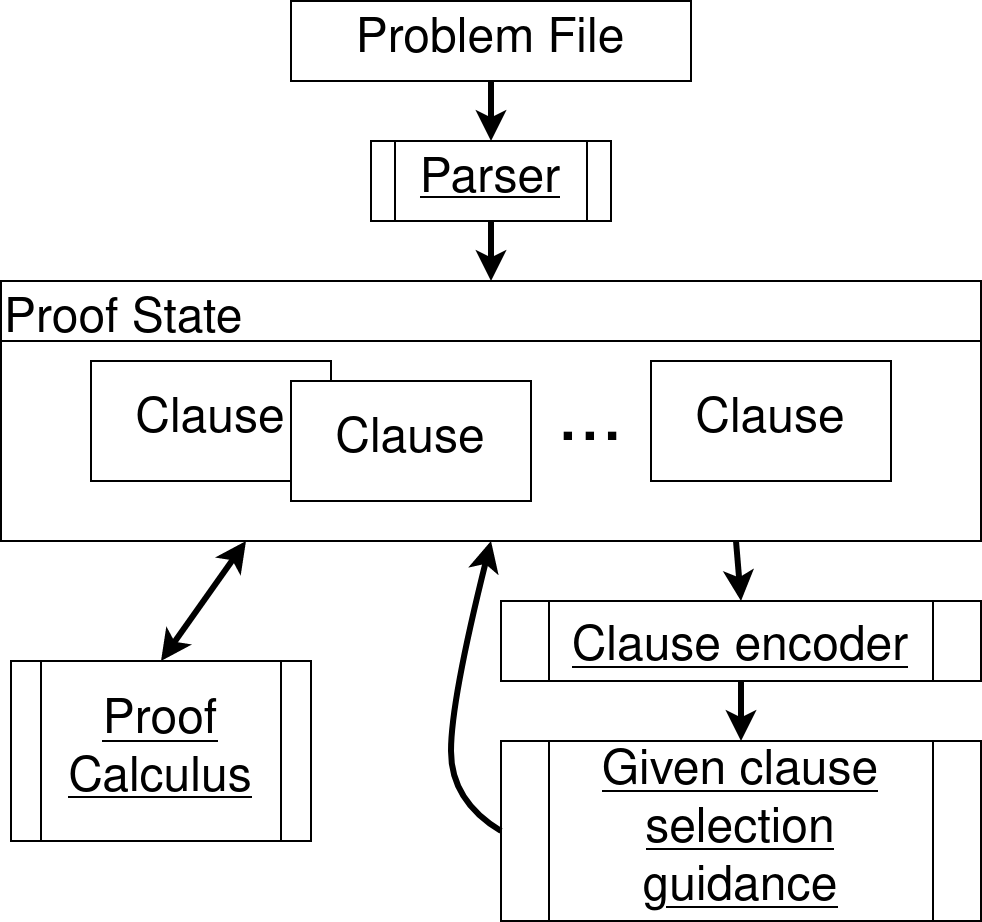
\includegraphics[scale=0.2]{SaturationProver}
\end{figure}
\end{frame}
\begin{frame}[t]
\frametitle{What about reinforcement learning?}
\begin{figure}
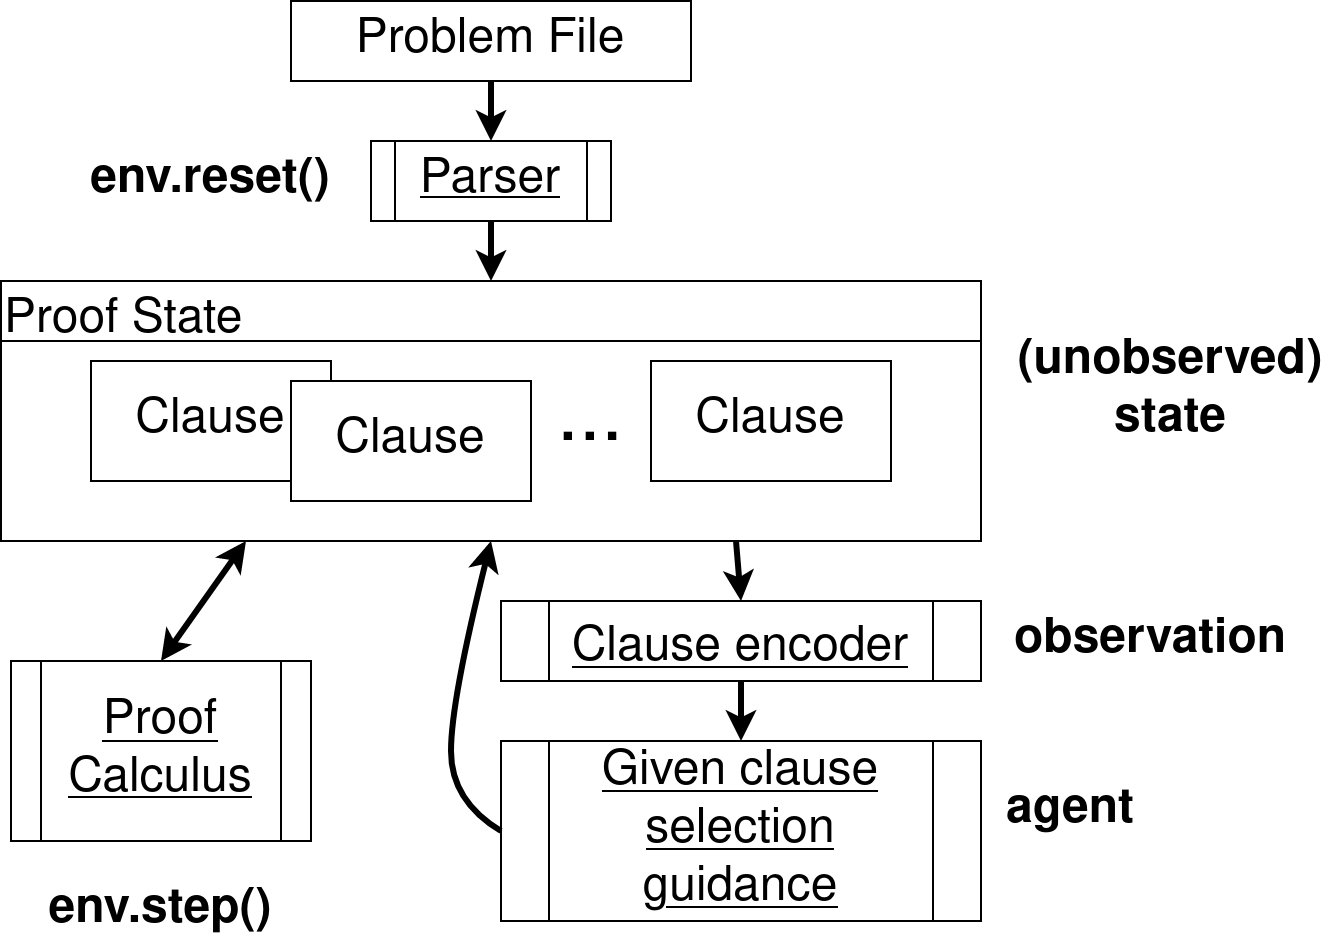
\includegraphics[scale=0.2]{RLSquint}
\end{figure}
\end{frame}
\begin{frame}[t]
\begin{figure}
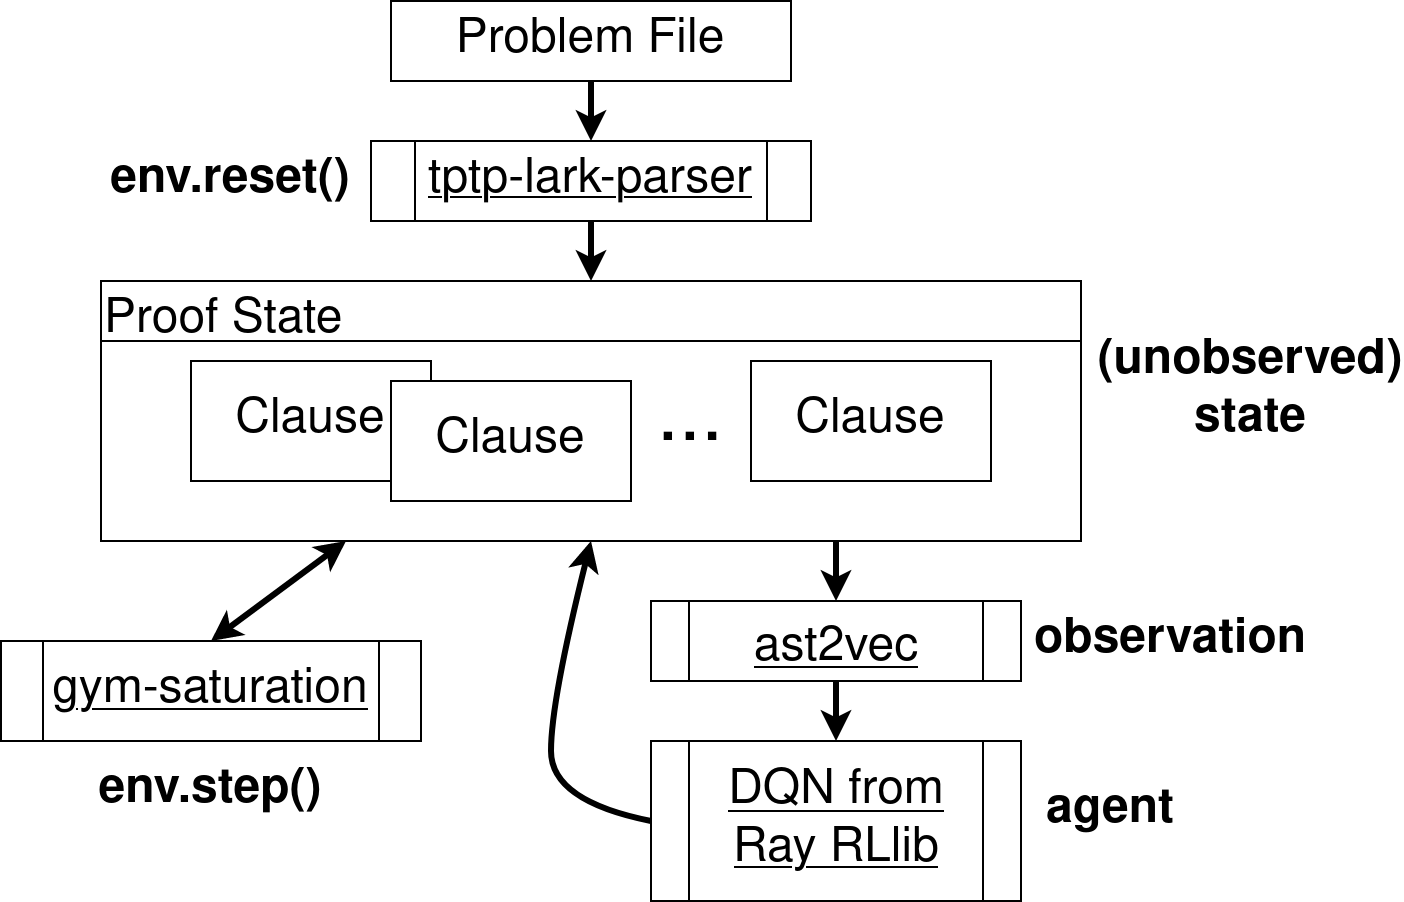
\includegraphics[scale=0.2]{Prototype}
\caption*{code available: \url{https://github.com/inpefess/basic-rl-prover}}
\end{figure}
\end{frame}
\begin{frame}[t]
\frametitle{Environment Demo}
\begin{figure}
\caption*{\url{https://bit.ly/3ccTbKv}}

\includegraphics[scale=0.3]{bit.ly_3ccTbKv}
\end{figure}
\end{frame}
\begin{frame}[t]
\frametitle{Independent Clauses Encoder (ast2vec)}
\begin{itemize}
\item a first order formula $\rightarrow$ Python code snippet $\rightarrow$ feature vector
\item a Docker container serving the model from B.~Paaßen, I.~Koprinska and K.~Yacef, Recursive tree grammar autoencoders. Mach Learn (2022)
\item code available \url{https://gitlab.com/inpefess/ast2vec}
\end{itemize}
\end{frame}
\begin{frame}[t]
\frametitle{What's next?}
\begin{itemize}
\item more agents: PPO (proximal policy optimization)
\item training/evaluation on a reasonable TPTP subset
\item CASC (Demonstration Division?)
\item more encoders (e.g. from S.~Purgał, J.~Parsert and C.~Kaliszyk, A study of continuous vector representations for theorem proving, in Journal of Logic and Computation, vol. 31, no. 8, pp. 2057-2083, Aug. 2021)
\end{itemize}
\end{frame}
\begin{frame}[t]
\frametitle{Thank you for your attention!}
\begin{itemize}
\item Discussion time!
\item More details and bibliography in the extended abstract \url{http://aitp-conference.org/2022/abstract/paper_2.pdf}
\item questions/criticism/collaboration proposals are welcome any time during the AITP 2022 and by the email \url{mailto:boris.shminke@univ-cotedazur.fr}
\end{itemize}
\end{frame}
\end{document}
